\documentclass[11pt]{article}

\usepackage[T1]{fontenc}
\usepackage[utf8]{inputenc}
\usepackage{lmodern}
\usepackage[a4paper,margin=1in]{geometry}
\usepackage{amsmath,amssymb,amsthm,mathtools}
\usepackage{booktabs}
\usepackage{array}
\usepackage{tabularx}
\usepackage{xcolor}
\usepackage{microtype}
\usepackage{enumitem}
\usepackage{listings}
\usepackage{tikz}
\usetikzlibrary{positioning,arrows.meta,calc}
\usepackage[hidelinks]{hyperref}

\setlength{\parindent}{0pt}
\setlength{\parskip}{0.55em}
\setlength{\emergencystretch}{3em}

\newtheorem{lemma}{Lemma}[section]
\newtheorem{theorem}[lemma]{Theorem}
\theoremstyle{definition}
\newtheorem{definition}[lemma]{Definition}
\newtheorem{example}[lemma]{Example}
\theoremstyle{remark}
\newtheorem{remark}[lemma]{Remark}

\lstset{basicstyle=\ttfamily\small,columns=fullflexible,keepspaces=true,
  frame=single,framerule=0.3pt,xleftmargin=1em,xrightmargin=1em,
  breaklines=true,breakatwhitespace=true,
  literate={<-}{{$\leftarrow$}}1 {->}{{$\rightarrow$}}2 {=>}{{$\Rightarrow$}}2}

\newcommand{\code}[1]{\texttt{#1}}
\newcommand{\file}[1]{\texttt{#1}}
\newcommand{\Start}{\mathit{Start}}
\newcommand{\sess}{\sigma}
\newcommand{\sol}[1]{\textbf{#1}}
\newcommand{\tok}[1]{\mathsf{#1}}
\newcommand{\Succ}{\mathsf{Succ}}
\newcommand{\pop}{\mathsf{pop}}
\newcommand{\trypop}{\mathsf{trypop}}
\newcommand{\push}{\mathsf{push}}
\newcommand{\startPop}{\mathsf{startPop}}
\newcommand{\getTop}{\mathsf{getTop}}
\newcommand{\tryRemove}{\mathsf{tryRemove}}
\newcommand{\newTS}{\mathsf{newTS}}
\newcommand{\gap}{\mathrm{gap}}
\newcommand{\TSTop}{\top}

\title{Supporting Elimination Compositionally in the TS Stack\\
  \large A verification plan for the \texttt{examples/TSStack} development}
\author{Prepared for Zhongye Wang}
\date{2026-10-27}

\begin{document}
\maketitle

\begin{abstract}
The timestamped stack of Dodds, Haas and Kirsch (POPL 2015) lets a pop
remove a node without finishing its scan when the node's timestamp is
later than the pop's own start time. Our development does not have this
\emph{elimination}. This document proposes how to add it while keeping
the layered structure: which interfaces change, what each specification
must say, how each implementation is written, what each layer proof has
to establish, in what order to do the work, and where the risk is. The
central decision is to move the atomic boundary from \code{trypop} to
\code{pop}: the start time and the retry loop live in one layer, whose
atomic specification is an atomic pop over the DAG. Everything below
ListPool and the DAG-to-list step above it are reused unchanged.
\end{abstract}

\tableofcontents

\section{Summary}

\sol{Goal.} Add the elimination mechanism of the original TS stack to
\file{examples/TSStack} and verify it down to plain memories and CAS
registers, producing a third top-level composition next to
\file{TSStack\_TopLevel.v} and \file{TSStack\_TopLevelUnlink.v}, with the
same axioms.

\sol{Decision.} Elimination changes \emph{where} a pop linearizes: an
eliminated node can be popped at a moment before the retry that performs
the elimination was even invoked (Section~\ref{sec:problem}). An atomic
\code{trypop} per retry therefore cannot be an intermediate specification
any more. The plan keeps the physical layer order and moves the atomic
boundary one layer down: the new layer \emph{DagStack} owns the start
time and the retry loop and is specified as an atomic pop over the DAG;
TryStackAux and ListPool become interval-sequential variants with a
pass-through \code{startPop} operation and an elimination rule; TSStack
keeps only the DAG-to-list step and loses its loop
(Figure~\ref{fig:layers}).

\sol{What is reused.} Timestamp, NodeMem, SPList (both variants),
SPListArray and SPListFamily are untouched, including their proofs. The
TSStack DAG-to-list argument (\code{I\_stack}, \code{I\_graph},
\code{I\_pending}, \code{G\_pop}) is reused with its loop removed. The
TryStack history theory (positions, legality, canonical history,
Lemma~A.1) is generalized rather than replaced.

\sol{What is new.} One abstract notion, the \emph{start set} of a pop
session (the vertices whose push had completed when the session started),
replaces timestamp comparison above ListPool. Two facts carry the
argument: a start-time comparison that succeeds implies the node is not
in the start set (proved once in ListPool, Lemma~\ref{lem:ts}), and a node
outside the start set has a moment inside the session at which it is a
top live vertex (proved once in the history theory,
Lemma~\ref{lem:window}).

\sol{Effort.} Six phases (Section~\ref{sec:phases}). The two large
items are the generalized history theory with the loop-owning DagStack
proof, and the ListPool scan with an early exit. The TryStackAux and
TSStack changes are moderate; the specifications and implementations
are small.

\begin{figure}[t]
\centering
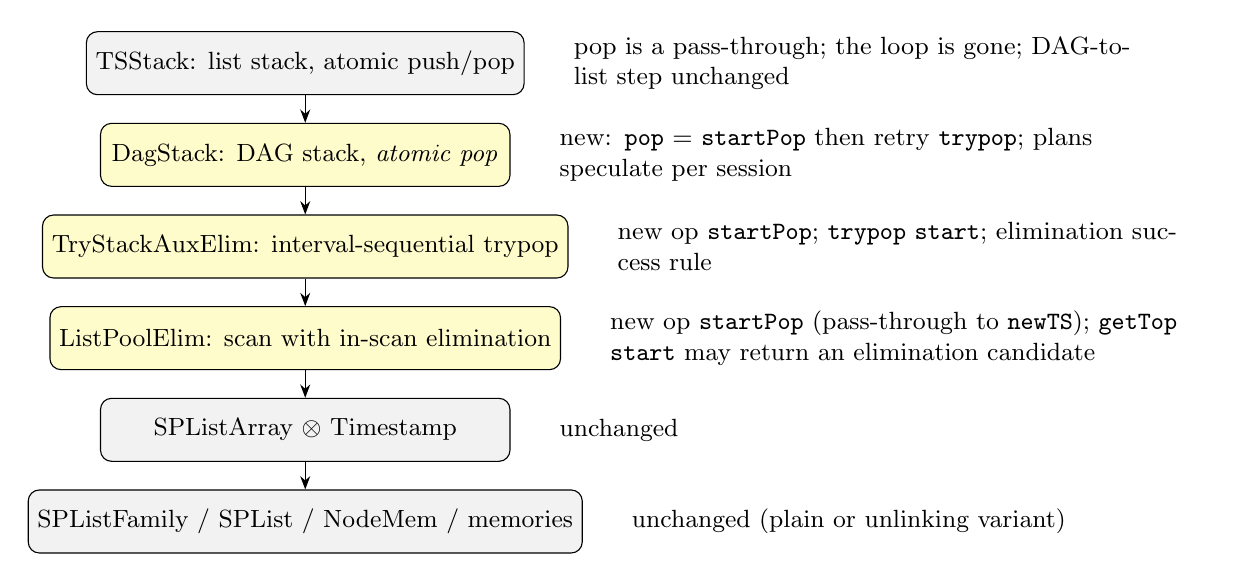
\begin{tikzpicture}[
  layer/.style={draw,rounded corners,minimum width=5.2cm,minimum height=0.8cm,align=center,font=\small},
  note/.style={font=\small,align=left,text width=7.2cm},
  >=Stealth]
  \node[layer,fill=gray!10] (ts) {TSStack: list stack, atomic push/pop};
  \node[layer,below=0.35cm of ts,fill=yellow!20] (dag) {DagStack: DAG stack, \emph{atomic pop}};
  \node[layer,below=0.35cm of dag,fill=yellow!20] (aux) {TryStackAuxElim: interval-sequential trypop};
  \node[layer,below=0.35cm of aux,fill=yellow!20] (lp) {ListPoolElim: scan with in-scan elimination};
  \node[layer,below=0.35cm of lp,fill=gray!10] (arr) {SPListArray $\otimes$ Timestamp};
  \node[layer,below=0.35cm of arr,fill=gray!10] (low) {SPListFamily / SPList / NodeMem / memories};
  \node[note,right=0.5cm of ts] {pop is a pass-through; the loop is gone; DAG-to-list step unchanged};
  \node[note,right=0.5cm of dag] {new: \code{pop} = \code{startPop} then retry \code{trypop}; plans speculate per session};
  \node[note,right=0.5cm of aux] {new op \code{startPop}; \code{trypop start}; elimination success rule};
  \node[note,right=0.5cm of lp] {new op \code{startPop} (pass-through to \code{newTS}); \code{getTop start} may return an elimination candidate};
  \node[note,right=0.5cm of arr] {unchanged};
  \node[note,right=0.5cm of low] {unchanged (plain or unlinking variant)};
  \draw[->] (ts) -- (dag); \draw[->] (dag) -- (aux); \draw[->] (aux) -- (lp); \draw[->] (lp) -- (arr); \draw[->] (arr) -- (low);
\end{tikzpicture}
\caption{The layer stack with elimination. Yellow layers are new variants; grey layers are reused as they are. The atomic boundary for pops is the DagStack interface, one layer lower than today's TryStack.}
\label{fig:layers}
\end{figure}

\section{Background}

\subsection{Elimination in the original algorithm}

In the original TS stack (Listing~2 of the paper), \code{pop} takes a
fresh timestamp once, before its retry loop, and passes it to every
retry:

\begin{lstlisting}
pop():
  startTime <- TS.newTimestamp()
  do { (ok, v) <- tryRem(startTime) } while (not ok)
  return v

tryRem(startTime):
  for each pool p (in some order):
    node <- p.getYoungest()
    if node = null then record p's top as empty-evidence; continue
    if startTime < node.timestamp then        // elimination
      return p.remove(node)                   // stop the scan here
    if maxTS < node.timestamp then remember node as the candidate
  if no candidate then return EMPTY if all empty-evidence still holds else FAIL
  return candidatePool.remove(candidate)
\end{lstlisting}

The comparison \code{startTime < node.timestamp} is the strict interval
order: the whole start interval precedes the whole node interval. The
unset timestamp $\TSTop$ of a node that has been inserted but not yet
stamped is larger than every interval, so such a node is eliminated too.
If the removal of the eliminated node fails (someone else took it),
\code{tryRem} fails and \code{pop} retries.

Why this is correct, informally: if the pop's start interval precedes the
node's interval, then the node's push had not completed when the pop
started, so the two operations overlap and the pop may be linearized
immediately after the push, at which moment the node is the top of the
stack.

\subsection{What the development has today}

\begin{center}
\small
\begin{tabularx}{\textwidth}{@{}lXl@{}}
\toprule
Layer & Spec / implementation / proof & Size of proof \\
\midrule
TSStack & \file{TSStackSpec.v}, \file{TSStack.v}, \file{TSStackProof.v} & 2.8k lines \\
TryStack & \file{TryStackSpec.v}, \file{TryStack.v}, \file{TryStackHistory.v}, \file{TryStackProof.v} & 1.6k + 4.7k \\
TryStackAux & \file{TryStackAuxSpec.v}, \file{TryStackAux.v}, \file{TryStackAuxProof.v} & 2.0k \\
ListPool & \file{ListPoolSpec.v}, \file{ListPool.v}, \file{ListPoolProof.v} & 11.0k \\
SPListArray, SPList(Unlink), NodeMem(Unlink), Timestamp & unchanged by this plan & \\
\bottomrule
\end{tabularx}
\end{center}

The pop of \file{TSStack.v} loops over the atomic \code{trypop} of
TryStack. TryStack's \code{trypop} is the atomic boundary: its
specification removes any top live vertex of the DAG, reports empty, or
fails, all at one instant inside the retry. The TryStack proof realizes
this with the plan machinery of the rewritten Appendix~A.4: ghost clocks
in TryStackAux, a canonical history $H$, and the set of all
\emph{plans} (legal histories that speculate at most one pop per pending
snapshot). The timestamp object is consumed only by ListPool's push.

\section{Why the current layering cannot host elimination}
\label{sec:problem}

\begin{example}[Elimination linearizes before the retry]
\label{ex:early}
Thread $\alpha$ starts a pop and obtains start time $[5,5]$. Then
thread $\beta_1$ pushes $n$ with timestamp $[6,6]$ and returns; thread
$\beta_2$ pushes $m$ with timestamp $[7,7]$ and returns, so $m$ is above
$n$ in the DAG (edge $m \to n$). Only now does $\alpha$'s first retry
run. It visits $n$'s pool first, sees $[5,5] < [6,6]$, and takes $n$.
\end{example}

The run is allowed by the original algorithm and is correct: the only
stack linearization places $\alpha$'s pop between the two pushes. That
instant lies before the retry was invoked. With the current TryStack
specification the retry's \code{trypop} would have to linearize inside
its own interval, where $n$ is not a top vertex because $m$ is live and
above it. So:

\begin{itemize}[nosep]
\item the atomic operation whose interval contains the linearization point
  is the whole \code{pop}, from \code{startPop} to the final return;
\item the layer that proves atomicity must see the start of the session
  and the retries as its own underlay events, so the retry loop must sit
  \emph{inside} that layer's implementation, not above it;
\item the layers below must expose the start of the session as an
  operation, so that their specifications can state what ``the push had
  not completed when the session started'' means without timestamps.
\end{itemize}

This fixes the design: the atomic boundary moves from \code{trypop} to
\code{pop}, the loop moves from TSStack into the new DagStack layer, and
\code{startPop} is threaded through TryStackAux and ListPool as a
pass-through operation whose abstract effect is to record a
\emph{start set}.

\section{The design}
\label{sec:design}

\subsection{The start set}

\begin{definition}[Start set]
When thread $\alpha$ invokes \code{startPop}, the specification records
\[
\Start[\alpha] \;=\; \{\, x \mid x \text{ is a vertex and its push is not pending}\,\}
\]
that is, the vertices whose push had completed at the invocation. The set
is recorded at the \emph{invocation}, not the response. A later
\code{startPop} by the same thread overwrites it.
\end{definition}

The start set is a ``completion snapshot'', the dual of the vertex
snapshot that \code{getTop} already records at its invocation
(\code{lp\_snapshots}). It plays the role of the marker vertex discussed
earlier: a marker with edges to every completed vertex has exactly
$\Start[\alpha]$ as its out-neighbourhood, and representing it as a set
avoids adding a vertex kind to every existing lemma about vertices.

\begin{definition}[Elimination rule, abstractly]
A pop session of $\alpha$ may remove vertex $n$ by elimination when $n$ is
live and $n \notin \Start[\alpha]$. No snapshot condition applies.
\end{definition}

\subsection{The two facts that carry the argument}

The first fact lives entirely in the ListPool proof and is the only place
timestamp values are compared.

\begin{lemma}[Start-time comparison implies non-membership]
\label{lem:ts}
Suppose $\alpha$'s \code{startPop} returned the interval $s=[l_s,u_s]$ and
a scan of $\alpha$ observed node $n$ with timestamp $t$ where
$s < t$ in the strict interval order (including $t=\TSTop$). Then
$n \notin \Start[\alpha]$.
\end{lemma}

\begin{proof}
If $n \in \Start[\alpha]$, then $n$'s push had completed at $\alpha$'s
\code{newTS} invocation, so $n$ carried a fixed interval $[l_n,u_n]$ at
that moment and still carries it (timestamps are written once). The
Timestamp specification records the clock at invocation as $l_s$, and a
completed \code{newTS} has raised the clock past its upper endpoint, so
$u_n < l_s$. The observed timestamp $t$ is therefore $[l_n,u_n]$, not
$\TSTop$, and $s < t$ means $u_s < l_n$. Together with $l_s \le u_s$ and
$l_n \le u_n$ this gives $u_n < l_s \le u_s < l_n \le u_n$, a contradiction.
\end{proof}

In Coq this is the invariant
\[
\forall n \in \Start[\alpha].\ \exists l\,u.\ \mathit{ts}(n) = [l,u] \wedge u < c_\alpha
\]
where $c_\alpha$ is the clock recorded by $\alpha$'s pending \code{newTS}
(\code{ts\_pending}) while the start is pending, and the lower endpoint
of the returned start interval afterwards. It is established at
\code{startPop} invocation from \code{stamped\_before\_clock} (already
in \file{ListPoolProof.v}) and is stable because timestamps are
immutable and the recorded clock does not change.

The second fact lives in the history theory and is the elimination case
of Lemma~A.1.

\begin{lemma}[Elimination window]
\label{lem:window}
Let $\sess_\alpha$ be the ghost clock of $\alpha$'s \code{startPop}
invocation and let $n$ be live with $n \notin \Start[\alpha]$, so either
$n$ is pending or its completion stamp $r(n)$ satisfies
$r(n) > \sess_\alpha$. Then there is a history position $P$ with
$\sess_\alpha < \gap(P) \le t$ (inside the session, not after the current
clock $t$), $n$ placed before $P$, and no vertex that is \emph{above} $n$
placed before $P$. Consequently the canonical history can be extended
with $\alpha$'s pop of $n$ at $P$ without postponing any push.
\end{lemma}

\begin{proof}
If $n$ is completed, take $P$ to be a fresh position at the very start of
gap $r(n)+1$, that is, right after the event that completed $n$. In a
legal history $n$ is placed at a gap $\le r(n) < \gap(P)$. A vertex $x$ is
above $n$ only if its placement gap exceeds $r(n)$, hence is at least
$\gap(P)$, and $P$ precedes every existing position of its gap, so no such
$x$ is placed before $P$. Finally $\sess_\alpha < r(n) < \gap(P) \le t$.
If $n$ is pending, nothing is above $n$ (``above'' needs a completion
stamp); take $P$ at the end of the current gap $t$, after $n$'s placement.
Legality, no-needless-delay and the other conclusions of Lemma~A.1 follow
as in the existing \code{ins\_canonical} proof with an empty blocker set.
\end{proof}

Lemma~\ref{lem:window} is strictly easier than the snapshot case of
Lemma~A.1, which has to postpone pending pushes that were placed above
the popped vertex. The two cases share the insertion construction.

\subsection{Session-based legality}

Today, legality (Fig.~31) ties every pop to a snapshot: a committed pop
of $n$ by $\beta$ at position $p$ requires $st < \gap(p) \le rt$ with
$st$ the snapshot time, and a speculative pop requires a pending snapshot
containing $n$. With sessions, the lower bound becomes the session start:

\begin{center}
\begin{tabular}{@{}ll@{}}
\toprule
Clause & New form \\
\midrule
(pop), committed & $M[n] = (\beta,\sess_\beta,rt)$ and $\sess_\beta < \gap(p) \le rt$ \\
(pop), speculative & $M[n]=\bot$, $\beta$ has an open session with start $\sess_\beta$, and $\sess_\beta < \gap(p)$ \\
(spec) & at most one speculative pop per thread (unchanged) \\
all other clauses & unchanged \\
\bottomrule
\end{tabular}
\end{center}

The snapshot is no longer part of legality. It is used only inside the
existence proof for a normal (non-elimination) removal, where the current
argument finds a position after the snapshot time $st$, and
$\sess_\beta < st$ holds because the session started before the retry.
The failing set $B$ and the relation \code{giveUpS} disappear: the atomic
pop has no fail result, so a failed retry linearizes nothing.

\subsection{What a plan speculates}

Today a plan speculates, for a pending snapshot, one pop at a position
after the snapshot of a vertex in the snapshot that is top there. The new
plan speculates, for an open session, one pop at a position after the
session start of a vertex that is live and top there in the plan's own
graph. The normal case is the special case where the position is after
the current retry's snapshot; the elimination case is the special case
where the vertex is outside the start set. Both are discharged by
Lemma~A.1 (generalized) at the moment the removal is reported.

\section{Specifications, layer by layer}
\label{sec:specs}

All new files are variants next to the existing ones, in the style of
the unlinking work (\file{SPListUnlink*.v}). The existing stack is not
modified. Suggested names are given; they are not important.

\subsection{ListPoolElim (\file{ListPoolElimSpec.v})}

Signature. \code{TS} from \file{TimestampSpec.v} is used as an opaque
token above ListPool; no layer above ListPool compares timestamps.

\begin{lstlisting}
Variant EListPool_op :=
| lpool_push (v : A)                  (* unchanged, ar unit *)
| lpool_startPop                      (* new, ar TS *)
| lpool_getTop (start : TS)           (* ar YResult, now takes the start token *)
| lpool_tryRemove (owner : tid) (loc : Addr).   (* unchanged *)
\end{lstlisting}

State: two maps are added to \code{ListPoolState}.

\begin{lstlisting}
lp_pop_starts : TMap.t LPNodeSet;   (* Start[actor], set at startPop invocation *)
lp_pop_ts     : TMap.t TS;          (* the token returned by the actor's startPop *)
\end{lstlisting}

Rules (prose; the Coq form follows the existing constructors).

\begin{itemize}[nosep]
\item \code{step\_startPop\_inv}: records
  $\Start[\alpha] = \{n \mid \code{is\_vertex}\ n \wedge \neg\code{is\_pending}\ n\}$
  and removes any previous token of $\alpha$. Control stays \code{LPReady}
  (interval-sequential, like push).
\item \code{step\_startPop\_res ts}: records $\code{lp\_pop\_ts}[\alpha] = ts$.
  Any \code{ts} is allowed; the specification does not interpret it.
\item \code{step\_getTop\_snapshot\_inv start} and
  \code{step\_getTop\_atomic\_inv start}: as today, with the extra premise
  $\code{lp\_pop\_ts}[\alpha] = \code{Some}\ start$.
\item \code{step\_getTop\_elim\_res}: from the snapshot branch, with
  $\code{lp\_pop\_starts}[\alpha] = \code{Some}\ N_0$,
  $\neg N_0\,n$ and $\code{lp\_vertices}\ s\ n = \code{Some}\ v$, respond
  \code{YSuccNode v (fst n) (snd n)} and clear the snapshot. Note the
  rule does not require $n$ live: the garbage response already covers the
  garbage case and keeping the rules overlapping avoids a case split in
  the scan proof.
\item \code{error\_getTop\_no\_session}: invoking \code{getTop start} when
  $\code{lp\_pop\_ts}[\alpha] \ne \code{Some}\ start$ is an error. This
  is what ties the argument to the recorded start set; the DagStack
  implementation always passes the token it just received, so the error
  never fires there.
\item All other rules are unchanged. The existing top-of-snapshot and
  garbage responses remain available for \code{getTop start}.
\end{itemize}

The result type is unchanged: an elimination candidate is reported as an
ordinary \code{YSuccNode}. The layer above cannot tell which rule produced
it and does not need to, because the two facts it may use (top of the
snapshot, or outside the start set) are both stable until its
\code{tryRemove}.

\subsection{TryStackAuxElim (\file{TryStackAuxElimSpec.v})}

Signature: \code{tsa\_push v}, \code{tsa\_startPop} (ar \code{TS}),
\code{tsa\_trypop (start : TS)} (ar \code{TResult}, unchanged result
type).

State: \code{tsa\_pop\_starts}, \code{tsa\_pop\_ts} as in ListPool, and
one ghost field \code{tsa\_session\_time : TMap.t nat}, the clock at the
session's \code{startPop} invocation. The removal log
\code{tsa\_removals} records \code{(remover, session time, removal time)}
instead of the snapshot time.

Rules.

\begin{itemize}[nosep]
\item \code{startPop} inv/res mirror ListPool's.
\item \code{tsa\_trypop start} invocation: snapshot branch or empty-atomic
  branch as today, plus the token premise.
\item \code{step\_tsa\_trypop\_succ} (snapshot top): as today; additionally
  \emph{closes the session} (removes the actor's start set, token and
  session time), because the retry loop ends on this result.
\item \code{step\_tsa\_trypop\_elim} (new): with
  $\code{tsa\_pop\_starts}[\alpha] = \code{Some}\ N_0$, $\neg N_0\,n$,
  $n$ live, value $v$: respond \code{TSuccNode v ...}, mark $n$ garbage,
  clear the snapshot, log the removal with the session time, close the
  session.
\item \code{step\_tsa\_trypop\_empty\_res}: closes the session.
\item \code{step\_tsa\_trypop\_fail}: keeps the session.
\item errors: actor outside the domain (as today); \code{trypop start}
  without a matching session.
\end{itemize}

Closing the session on the terminal results is what makes ``$\beta$ has an
open session'' coincide with ``$\beta$ is inside a pop'' for the layer
above, so plans speculate only for threads that are inside a pop.

\subsection{DagStack (\file{DagStackSpec.v}), the new atomic boundary}

Signature: \code{dag\_push v} (ar \code{unit}), \code{dag\_pop}
(ar \code{PopResult}) with
\begin{lstlisting}
Variant PopResult := PNode (v : A) (owner : tid) (loc : Addr) | PEmpty.
\end{lstlisting}
The vertex identity stays in the result because the TSStack filter
(departure~2 of \file{TSStackVerificationPlan.md}) keys on it.

State: \code{TryStackState} of \file{TryStackSpec.v} as it is
($V,E,P,g$). Control: \code{Ready} / \code{AtomicPending} as in
TryStack.

Rules: push inv/res as in TryStack; \code{pop} invocation moves to
\code{AtomicPending}; \code{pop\_succ} removes any top live vertex
(\code{lp\_top (ts\_is\_live s) (ts\_edges s) n}); \code{pop\_empty}
requires all vertices garbage. There is \emph{no fail rule}. This is
\file{TryStackSpec.v} with \code{trypop} renamed and the fail
constructor deleted.

\subsection{TSStackElim}

\file{TSStackSpec.v} is reused as the overlay. Only the implementation
changes (next section). The specification of the whole stack is the same
atomic list stack as before, so the top-level theorem reads exactly like
\file{TSStack\_TopLevel.v}.

\section{Implementations}
\label{sec:impls}

\subsection{ListPoolElim (\file{ListPoolElim.v})}

\begin{lstlisting}
startPop_impl := inr newTS >= ts => Ret ts.

getTop_impl (start : TS) :=
  inl array_resetIter >= _ =>
  From (ThreadDomain.threads D, (None, 0)) Do { '(remaining, scan) =>
    match remaining with
    | nil => Break (inr scan)
    | owner :: rest =>
        inl (array_getTop owner) >= result =>
        match result with
        | inl (v, ts, loc) =>
            if timestamp_ltb start ts
            then Break (inl (v, owner, loc))                     (* elimination *)
            else Continue (rest, (choose_candidate owner (v,ts,loc) (fst scan), snd scan))
        | inr count => Continue (rest, (fst scan, snd scan + count))
        end
    end } Loop >= r =>
  match r with
  | inl (v, owner, loc) => Ret (YSuccNode v owner loc)
  | inr scan => (* exactly today's post-scan code: candidate, or counter check *)
  end.
\end{lstlisting}

The scan becomes a \code{From ... Do \{ \} Loop} over the unvisited
suffix so that it can \code{Break}. This is the idiom already used by
\code{skip\_taken\_impl} in \file{SPListUnlink.v}, and
\code{provable\_doloop\_data} is its proof rule. The accumulator carries
the suffix explicitly because the loop rule has no built-in iteration
variable. Push and \code{tryRemove} are unchanged.

\begin{remark}[Alternative without a new loop form]
Keep \code{ForEach} and add an ``eliminated'' flag to the accumulator;
once set, \code{scan\_step} returns immediately without any underlay
call. The underlay trace is identical to the early exit. This keeps
\code{provable\_foreach} and the existing \code{ScanFold} skeleton at the
cost of a three-mode accumulator. Choose this if restructuring the scan
proof around \code{provable\_doloop\_data} turns out to be more work than
expected (Section~\ref{sec:risks}).
\end{remark}

\subsection{TryStackAuxElim (\file{TryStackAuxElim.v})}

\begin{lstlisting}
startPop_impl := lpool_startPop >= ts => Ret ts.
trypop_impl (start : TS) :=
  lpool_getTop start >= result =>
  match result with
  | YSuccNode v owner loc => lpool_tryRemove owner loc >= removed =>
                             Ret (if removed then TSuccNode v owner loc else TFail)
  | YSuccEmpty => Ret TSuccEmpty
  | YFail => Ret TFail
  end.
\end{lstlisting}
Identical to today except for the pass-through and the argument. The
removal of an elimination candidate happens here, as the removal of a
normal candidate does today. The original performs it inside the scan
function; the sequence of underlying operations is the same.

\subsection{DagStack (\file{DagStack.v})}

\begin{lstlisting}
push_impl v := tsa_push v >= _ => Ret tt.
pop_impl :=
  tsa_startPop >= start =>
  Do { tsa_trypop start >= r =>
       Ret (match r with
            | TSuccNode v o l => inr (PNode v o l)
            | TSuccEmpty      => inr PEmpty
            | TFail           => inl tt end) } Loop.
\end{lstlisting}
This is today's \file{TSStack.v} pop with \code{startPop} in front and
TryStackAuxElim as the underlay.

\subsection{TSStackElim (\file{TSStackElim.v})}

\begin{lstlisting}
push_impl v := dag_push v >= _ => Ret tt.
pop_impl := dag_pop >= r => Ret (match r with PNode v _ _ => Some v | PEmpty => None end).
\end{lstlisting}

\section{Proof plan, layer by layer}
\label{sec:proofs}

\subsection{ListPoolElimProof}

Starting point: a copy of \file{ListPoolProof.v}. The set logic,
\code{I}, \code{R}, \code{G} and the push and \code{tryRemove} proofs are
kept.

\begin{enumerate}[nosep]
\item \sol{Invariant.} Add to the per-branch representation that
  \code{lp\_pop\_starts} and \code{lp\_pop\_ts} agree with the concrete
  state as follows: the start-set clause of Lemma~\ref{lem:ts} (every
  member is stamped with an interval whose upper endpoint is below the
  actor's recorded clock), and the token equals the actor's last
  \code{newTS} result while no \code{newTS} of the actor is pending. Both
  maps are uniform across branches (vertices and pending pushes already
  are).
\item \sol{Rely/guarantee.} Other threads never change my start set or
  token; my own \code{startPop} replaces both. Add this to
  \code{array\_evolves}-style clauses; the existing \code{R} already says
  that other threads' pushes only add vertices.
\item \sol{startPop.} Invocation: \code{pstep} the deterministic
  \code{step\_startPop\_inv} in every branch (uniform). Then the
  underlay \code{newTS} inv/res; the response value is recorded by
  \code{step\_startPop\_res}. The Timestamp facts needed are the ones
  push already uses (\code{start\_newTS\_records\_clock},
  \code{finish\_newTS\_clock\_past}, \code{stamped\_before\_clock}).
\item \sol{getTop, token premise.} At invocation, \code{provable\_perror}
  with the new error; otherwise the token matches in every branch.
\item \sol{getTop, scan loop.} Re-prove the scan under
  \code{provable\_doloop\_data} with the loop data \code{(remaining, scan)}
  and the invariant \code{ScanFold actor remaining scan}, which is
  already indexed by the unvisited suffix. The \code{Continue} branches
  are today's fold step. The new \code{Break} branch on
  \code{timestamp\_ltb start ts = true} must establish the elimination
  precondition $\neg\Start[\alpha]\,n$ from Lemma~\ref{lem:ts} and the
  vertex's existence; it needs none of the visited/ignored bookkeeping.
\item \sol{getTop, elimination response.} Commit the possibility set to
  the snapshot branches and apply \code{step\_getTop\_elim\_res} in each
  (uniform, since it depends only on the start set and the vertex map).
  This is simpler than the top-of-snapshot response, which needs the
  witness invariant over the visited rows.
\item \sol{Stale $\TSTop$.} An observed $\TSTop$ is eliminated. The
  obligation is again $\neg\Start[\alpha]\,n$: a member of the start set
  carries an interval, so it cannot be observed as $\TSTop$.
\end{enumerate}

Acceptance: \code{MListPoolElim} and \code{MListPoolElimLinearizable}
with the same statement shape as today; no \code{Admitted}; the
timestamp comparison appears in no lemma outside this file and
\file{ListPoolElim.v}.

\subsection{TryStackAuxElimProof}

Starting point: a copy of \file{TryStackAuxProof.v} (singleton facade).

\begin{enumerate}[nosep]
\item \sol{Graph invariant.} \code{graph\_represents} additionally equates
  the start sets, tokens and (one-directionally) the session bookkeeping
  of the two isomorphic states. The ghost session time is a function of
  the pre-state and the event and never constrains a step, like the other
  ghost fields.
\item \sol{startPop.} Lock-step pass-through: ListPool inv $\mapsto$
  TSA inv, ListPool res $\mapsto$ TSA res.
\item \sol{trypop.} After \code{getTop start} returns \code{YSuccNode},
  invert the ListPool step: top-of-snapshot, garbage, or elimination.
  Carry the corresponding stable fact to \code{tryRemove}: ``$n$ top of
  my snapshot among live'' (stable under garbage growth while $n$ is
  live, as today), or ``$n \notin \Start[\alpha]$'' (stable, start sets
  never change). On \code{tryRemove} success apply
  \code{step\_tsa\_trypop\_succ} or \code{step\_tsa\_trypop\_elim}
  respectively; the garbage case cannot succeed. On failure apply the
  fail rule, which keeps the session.
\item \sol{Session closing.} The success and empty responses close the
  session in both states; the invariant needs ``session open in ListPool
  iff open in TSA''.
\end{enumerate}

Acceptance: \code{MTryStackAuxElim}, \code{MListPoolTryStackAuxElim}
(vertical composition with ListPoolElim).

\subsection{DagStackHistory (generalized \file{TryStackHistory.v})}

This is the mathematical core and should be done \emph{before} the layer
proofs that depend on it (Section~\ref{sec:phases}).

\begin{enumerate}[nosep]
\item \sol{Ghost well-formedness.} Extend \code{ghost\_wf} with the
  session clauses: $\Start[\alpha] = \{x \mid \exists r_x.\ r(x) = r_x \wedge r_x < \sess_\alpha\}$
  for every open session, $\sess_\alpha < t$, and
  $\sess_\alpha < \tau(\alpha)$ whenever $\alpha$ also has a pending
  snapshot. Prove preservation for the new events (\code{startPop}
  inv/res) and the session-closing responses.
\item \sol{Legality.} Replace the snapshot bound in \code{lg\_pop} by the
  session bound (table in Section~\ref{sec:design}); drop the
  $N\,n$ requirement from the speculative disjunct. Re-check every lemma
  that unfolds \code{lg\_pop}; the \code{ins\_*} lemmas of the insertion
  construction are the main consumers.
\item \sol{Lemma A.1, normal case.} Keep \code{slot\_exists} as it is; its
  conclusion $st < \gap(Q)$ now implies the session bound through
  $\sess_\alpha < st$.
\item \sol{Lemma A.1, elimination case.} New \code{slot\_exists\_elim}
  from Lemma~\ref{lem:window}: fresh position at the start of gap
  $r(n)+1$ (use \code{rank\_below}) or at the end of the current gap (use
  \code{rank\_above}), empty blocker set. Instantiate the existing
  \code{Section Slot} with it; \code{ins\_canonical} should go through
  with the blocker hypotheses trivially satisfied.
\item \sol{Statement.} \code{fs\_insertion} takes a disjunctive premise:
  ($\tau(\alpha)=st$, $S[\alpha]=N$, $n$ top of $N\setminus g$) or
  ($n$ live, $n \notin \Start[\alpha]$); it concludes
  $\sess_\alpha < \gap(P) \le t$ instead of $st < \gap(P) \le t$.
\end{enumerate}

Acceptance: the file compiles with \code{Print Assumptions} showing only
\code{classic}, as today.

\subsection{DagStackProof (generalized \file{TryStackProof.v})}

Starting point: a copy of \file{TryStackProof.v}. Tokens are for
\code{dag\_pop}: $\tok{\circ(pop)}$, $\tok{\bullet(pop,\Succ(v,n))}$,
$\tok{\bullet(pop,\bot)}$; there is no fail token.

\begin{enumerate}[nosep]
\item \sol{Representation and plans.} \code{rep\_tokens}: for every
  thread $\beta$ with an open session, the token is
  $\tok{\bullet(pop,\Succ(v,n))}$ if the plan has a speculative pop of
  $n$ by $\beta$ and $\tok{\circ(pop)}$ otherwise. The failing set $B$
  and its clause are removed. \code{plan s H h} keeps (P2), (P3).
\item \sol{Lag.} In \code{lag}, the clause ``$n \in g_p \setminus g$ is
  justified by a pending snapshot containing $n$'' becomes ``justified by
  an open session of a thread whose token is
  $\tok{\bullet(pop,\Succ(V[n],n))}$''.
\item \sol{Speculation.} \code{popS}: session open, token
  $\tok{\circ(pop)}$, $n$ live and top in the possibility's own graph;
  the $N\,n$ premise is dropped. \code{giveUpS} is deleted;
  \code{specS} is the closure of \code{placeS} and \code{popS}. Re-prove
  \code{plans\_reached} (plans with events in the current gap are reached
  by speculation): the induction is unchanged, the base case no longer
  needs \code{giveUpS}.
\item \sol{Guarantees.}
  \code{G\_start\_inv}: concrete \code{startPop} invocation with
  $\alpha \mapsto \tok{\circ(pop)}$ everywhere, then \code{specS}
  (as \code{G\_snap}).
  \code{G\_start\_ret}: concrete response, $\Delta$ unchanged, then
  \code{specS}.
  \code{G\_snap}: unchanged.
  \code{G\_fail}: concrete fail response with $\Delta$ unchanged, then
  \code{specS}; no filter (the retry linearizes nothing).
  \code{G\_rmv}: as today, with the enabledness from the generalized
  Lemma~A.1 in either case.
  \code{G\_emp}: as today, with the session closed in $\sigma'$.
  \code{G\_push\_inv}, \code{G\_push\_ret}: unchanged.
\item \sol{Outline of pop.} \code{provable\_doloop} around the retry with
  the loop assertion
  \[
  I \wedge \alpha \mapsto_\forall \tok{\circ(pop)} \wedge \text{session of } \alpha \text{ open} \wedge S[\alpha] = \bot .
  \]
  The retry body is today's \code{trypop} outline with the intermediate
  assertion $I \wedge S[\alpha] \ne \bot$ and the response update selected
  by the result: fail returns to the loop assertion, success and empty
  yield $I \wedge \alpha \mapsto_\forall \tok{\bullet(pop,r)}$ and break.
  The pre-loop \code{startPop} establishes the loop assertion from
  $I \wedge \alpha \mapsto_\forall \tok{\circ(pop)} \wedge$ no session.
\item \sol{Stability.} The loop assertion is stable because other
  threads never touch my session, and \code{specS} by others preserves
  my $\tok{\circ(pop)}$ token in some possibility (the plan with no
  speculation for me).
\end{enumerate}

Acceptance: \code{MDagStack}, \code{MDagStackLinearizable},
\code{MListPoolDagStack} (composition down to ListPoolElim's underlay);
assumptions \code{classic} and \code{Eq\_rect\_eq} for the layer proof.

\subsection{TSStackElimProof}

Starting point: a copy of \file{TSStackProof.v}. The pop method becomes a
single \code{provable\_vis\_safe} with the existing \code{PopAtomic} and
\code{PopPost} assertions; the \code{provable\_doloop} wrapper and the
\code{TFail} branch of \code{trypop\_res\_update} are deleted. The
relations \code{G\_pop}, \code{G\_pop\_emp}, \code{G\_push\_inv},
\code{G\_push\_ret} and the invariants are unchanged; only the underlay
constructor names change. Expect mostly deletions.

\subsection{Top-level composition}

\file{TSStack\_TopLevelElim.v} mirrors \file{TSStack\_TopLevel.v}:
\begin{center}
memories and CAS $\triangleright \ldots \triangleright$ \code{MListPoolElim} $\triangleright$ \code{MTryStackAuxElim}\\
$\triangleright$ \code{MDagStack} $\triangleright$ \code{MTSStackElim}.
\end{center}
Because SPListArray's interface is untouched, the same file can be
instantiated with \file{SPListUnlinkFamily.v} to obtain a stack with
both unlinking and elimination; call that file
\file{TSStack\_TopLevelElimUnlink.v}.
Acceptance: \code{Print Assumptions} equals that of the existing
top-level theorems.

\section{Work plan}
\label{sec:phases}

\subsection{Phases and order}

\begin{enumerate}
\item \sol{Specifications and implementations} (small). Write
  \file{ListPoolElimSpec.v}, \file{ListPoolElim.v},
  \file{TryStackAuxElimSpec.v}, \file{TryStackAuxElim.v},
  \file{DagStackSpec.v}, \file{DagStack.v}, \file{TSStackElim.v}; register
  in \file{\_CoqProject}; build. Freeze the specifications before any
  proof starts, since phases 2 to 4 depend on them and can then run in
  parallel.
\item \sol{History theory} (large, highest risk). \file{DagStackHistory.v}:
  session-based legality, generalized Lemma~A.1 with the elimination
  case. This is the ``extend Appendix~A.4 first'' step, done directly in
  Coq against the frozen TryStackAuxElim specification. Stop and report
  if session-based legality breaks any \code{ins\_*} lemma in a way the
  argument of Lemma~\ref{lem:window} does not cover.
\item \sol{ListPoolElimProof} (large, mostly mechanical). Independent of
  phase 2.
\item \sol{TryStackAuxElimProof} (medium). Independent of phase 2.
\item \sol{DagStackProof} (large). Depends on phase 2.
\item \sol{TSStackElimProof, top level, documentation} (small). Write
  the markdown plan in \file{docs/plans} with the departures recorded,
  update \file{docs/README.md}, and add pitfalls met to
  \file{docs/CoqPitfalls.md}.
\end{enumerate}

\subsection{Size estimates}

Sizes are relative to the files being copied; they are rough.

\begin{center}
\small
\begin{tabularx}{\textwidth}{@{}>{\raggedright\arraybackslash}p{3.3cm}>{\raggedright\arraybackslash}p{3.0cm}Xl@{}}
\toprule
File & Based on & Expected change & Size \\
\midrule
ListPoolElimSpec, ListPoolElim & ListPoolSpec, ListPool & +2 maps, +4 rules, +1 error; loop rewrite & small \\
TryStackAuxElimSpec, TryStackAuxElim & TryStackAuxSpec, TryStackAux & +3 maps, +1 rule, session closing & small \\
DagStackSpec, DagStack & TryStackSpec, TSStack & rename, delete fail, add startPop+loop & small \\
TSStackElim & TSStack & delete loop & trivial \\
DagStackHistory & TryStackHistory (1.6k) & legality, ghost\_wf, A.1 elim case & +15--25\% \\
ListPoolElimProof & ListPoolProof (11k) & start-set invariant, startPop, scan loop rewrite & +5--10\%; scan re-proved \\
TryStackAuxElimProof & TryStackAuxProof (2k) & pass-through, elim case, sessions & +20\% \\
DagStackProof & TryStackProof (4.7k) & sessions, no $B$, startPop guarantees, loop & $\pm$10\%; large churn \\
TSStackElimProof & TSStackProof (2.8k) & delete loop and fail branch & $-$5\% \\
Top level & TSStack\_TopLevel & composition & trivial \\
\bottomrule
\end{tabularx}
\end{center}

\subsection{Risks and mitigations}
\label{sec:risks}

\begin{itemize}
\item \sol{The scan loop rewrite in ListPool.} The scan proof is the
  largest proof in the development and is written against
  \code{provable\_foreach}. Switching to \code{provable\_doloop\_data}
  touches the whole \code{ScanFold} section. Mitigation: the flag
  alternative in Section~\ref{sec:impls} keeps \code{ForEach}; decide
  after reading how \code{ScanFold} is consumed at lines
  10731--10780 of \file{ListPoolProof.v}.
\item \sol{Session-based legality.} The existing \code{ins\_*} lemmas use
  $st < \gap(Q)$ in places where the session bound is now needed; most
  follow from $\sess_\alpha < st$, but any lemma that uses the snapshot
  membership $N\,n$ of a speculative pop needs a new argument. Mitigation:
  do phase 2 first and report blockers before touching DagStackProof.
\item \sol{Plans for threads outside a pop.} Speculation must not invent
  pops for threads that are not inside a pop. The session-closing rules
  make this a state property; make sure no path leaves a session open
  after a terminal result (both the success and empty rules close it).
\item \sol{Token mismatch errors.} The new error rules are needed for
  soundness of ListPoolElim and TryStackAuxElim as stand-alone layers;
  DagStack discharges them by \code{provable\_perror} with the token it
  received. Keep the token in the DagStack outline assertion.
\item \sol{Ghost clock conventions.} Coq stamps events with the pre-state
  clock; the dictionary in \file{TryStackVerificationPlan.md} applies,
  with $\sess_\alpha$ the stamp of the \code{startPop} invocation.
\end{itemize}

\section{Departures from the original and rejected alternatives}

\subsection{Departures to record}

\begin{enumerate}[nosep]
\item The elimination candidate is returned by \code{getTop} and removed
  by TryStackAux's \code{tryRemove}, instead of being removed inside the
  scan function. The sequence of array operations is the same and a
  failed removal fails the retry in both versions.
\item The scan visits pools in the fixed order of the thread domain, as
  today.
\item The counter-based emptiness check is kept (it is independent of
  elimination).
\item No timestamping delay; TS-CAS only; no memory reclamation, as
  today.
\item The start token is passed explicitly through the interfaces as a
  \code{TS} value, with an error when it does not match the recorded
  session. The original keeps it in a local variable; our layers have no
  local state across calls.
\end{enumerate}

\subsection{Rejected alternatives}

\begin{itemize}
\item \sol{Keep an atomic \code{trypop} and give it a history-carrying
  specification} (``the popped vertex was top at some moment since the
  session began''). Expressible, but it pushes the prophecy into the
  TSStack proof while the plan machinery stays one layer down; both
  proofs get harder.
\item \sol{Take the start time inside each retry.} Then the marker
  coincides with the snapshot, today's TryStack and TSStack proofs survive,
  and only ListPool, TryStackAux and the plan proof change. But under
  contention later retries eliminate fewer nodes than the original: a
  weaker heuristic, not the original algorithm. Keep as a fallback only if
  the user accepts the behavioral change.
\item \sol{Expose the Timestamp object horizontally} so that DagStack
  calls \code{newTS} directly. The Timestamp object is already consumed by
  ListPool's implementation; the framework's horizontal composition
  partitions underlay state and cannot share an object between a
  component implementation and a pass-through. The pass-through
  \emph{operation} with an abstract start set is the compositional form
  of the same idea.
\item \sol{Marker vertices in the vertex map.} Equivalent to the start
  set, but every lemma about vertices would need a case for the new kind.
\item \sol{A new result constructor \code{YSuccElim}.} Not needed: the
  layer above inverts the underlay step anyway, and keeping the result
  type avoids touching TryStackAux's result handling.
\end{itemize}

\appendix

\section{Dictionary of changes}

\begin{center}
\small
\begin{tabularx}{\textwidth}{@{}>{\raggedright\arraybackslash}p{3.6cm}>{\raggedright\arraybackslash}p{4.2cm}X@{}}
\toprule
Concept & Today & With elimination \\
\midrule
atomic pop boundary & TryStack \code{trypop} & DagStack \code{pop} \\
retry loop & \file{TSStack.v} & \file{DagStack.v} \\
start of a pop & none & \code{startPop} (ListPool, TryStackAux), returns \code{TS} \\
eligibility for elimination & none & $n \notin \Start[\alpha]$ \\
timestamp comparison & ListPool scan (candidate choice) & ListPool scan (candidate choice and elimination) \\
pop lower bound in legality & snapshot time $st$ & session time $\sess_\alpha$ \\
speculative pop condition & $n \in S[\beta]$, top & session open, top \\
failing set $B$, \code{giveUpS} & present & removed \\
removal log entry & (remover, $st$, $rt$) & (remover, $\sess$, $rt$) \\
fail token $\tok{\bullet(trypop,Fail)}$ & present & none (no fail at the atomic level) \\
\bottomrule
\end{tabularx}
\end{center}

\section{Checklist}

\begin{itemize}[nosep]
\item[$\square$] Specifications frozen; all implementations build.
\item[$\square$] \code{ghost\_wf} with sessions preserved by every TryStackAuxElim step.
\item[$\square$] Session-based legality; \code{fs\_insertion} with both cases; \code{classic} only.
\item[$\square$] ListPoolElim: start-set invariant; \code{startPop}; scan with early exit; elimination response.
\item[$\square$] TryStackAuxElim: pass-through; three-way inversion after \code{getTop}; session closing.
\item[$\square$] DagStack: plans without $B$; \code{plans\_reached}; guarantees incl.\ \code{G\_start\_*}; loop outline.
\item[$\square$] TSStackElim: loop removed; composition; \code{Print Assumptions} unchanged.
\item[$\square$] Optional: \file{TSStack\_TopLevelElimUnlink.v}.
\item[$\square$] Plan markdown, README row, pitfalls entries.
\end{itemize}

\end{document}
